\documentclass[10pt,twocolumn]{article}

\usepackage{amsmath}
\usepackage{bold-extra}
\usepackage{color}
\usepackage{epic}
\usepackage{float}
\usepackage{graphicx}
\usepackage{listings}
\usepackage{subfigure}
\usepackage{url}

%%%%%%%%%%%%%%%
%%% Colours %%%
%%%%%%%%%%%%%%%

\definecolor{darkgreen}{rgb}{0, 0.6, 0}
\definecolor{lightgrey}{gray}{0.9}

%%%%%%%%%%%
% Figures %
%%%%%%%%%%%

\newcommand{\stufigex}[5]					% images with specified placement
{
	\begin{figure}[#5]
	\begin{center}
		\includegraphics[#1]{#2}
		\caption{#3}
		\label{#4}
	\end{center}
	\end{figure}
}

% Define the stusubfig environment
\newenvironment{stusubfig}[1]
{
	\begin{figure*}[#1]
	\begin{center}
}
{
	\end{center}
	\end{figure*}
}

%%%%%%%%%%%%%%%%%
% Code Listings %
%%%%%%%%%%%%%%%%%

% Create a new type of float (called a stulisting) for listings
\floatstyle{ruled}
\newfloat{stulisting}{thp}{lop}
\floatname{stulisting}{Listing}

% Setup before using the listings package
\renewcommand{\lstlistingname}{\textbf{Listing}}
\def\thelstlisting{\textbf{\arabic{lstlisting}}}

\lstdefinelanguage{Pseudocode}{
morekeywords={and,assert,break,case,continue,default,down,each,else,for,function,if,not,null,or,rangeswitch,ref,return,switch,then,this,throw,to,up,var,while},
sensitive=true,
morecomment=[l]{//},
morecomment=[s]{/*}{*/}
}

\lstdefinestyle{Default}{
abovecaptionskip=0.5cm,
basicstyle=\scriptsize\ttfamily,
belowcaptionskip=0.5cm,
belowskip=0.5cm,
columns=fixed,
%commentstyle=\color{darkgreen},
commentstyle=\textit, % changed from the thesis (green text looks unprofessional in a journal paper)
language=Pseudocode,
%numbers=left,
numbers=none, % changed from the thesis (line numbers are less relevant here)
numbersep=5pt,
numberstyle=\tiny,
mathescape=true,
showstringspaces=false,
stepnumber=1,
tabsize=4
}

\lstdefinestyle{Snippet}{
abovecaptionskip=0.5cm,
aboveskip=0.5cm,
basicstyle=\small\ttfamily,
belowcaptionskip=0.5cm,
belowskip=0.5cm,
columns=fixed,
commentstyle=\color{darkgreen},
frame=lines,
keywordstyle=\small\bfseries,
language=Pseudocode,
numbers=none,
mathescape=true,
showstringspaces=false,
stepnumber=1,
tabsize=4
}

% For C++ function prototypes
\lstdefinestyle{Prototype}{
abovecaptionskip=0.5cm,
basicstyle=\small\ttfamily,
belowcaptionskip=0.5cm,
belowskip=0.5cm,
columns=fixed,
commentstyle=\color{darkgreen},
language=C++,
numbers=none,
mathescape=true,
showstringspaces=false,
stepnumber=1,
tabsize=4
}

%%%%%%%%%%%%%%%%%
% Main Document %
%%%%%%%%%%%%%%%%%

\begin{document}

\title{Object-Environment Collision Detection using Onion BSPs}
\author{Stuart Golodetz}
\date{}
\maketitle

\section{Introduction}

In my last article \cite{golodetzoverload13oct}, I described how to automatically generate navigation meshes to support the navigation of agents around 3D environments (e.g.~game worlds), as implemented in my homemade \emph{hesperus} engine \cite{hesperus}. However, there is far more to such navigation than simply mesh generation: it remains to be shown how to determine where (if anywhere) an agent can be found on the mesh and how to make best use of the mesh when allowing both user-controlled and AI agents to move around the environment. Agent movement must necessarily interact with an implementation's physics system, since the navigation mesh only covers the \emph{walkable} surfaces of the world and there is a need to ensure that agents are simulated correctly even when they are not on the mesh. In particular, any implementation needs to ensure that agents do not collide with either the world or each other, and that the effects of forces such as gravity are properly applied to them when not on the mesh. For that reason, before tackling the agent movement problem itself, it is important to take a step back and look at how to implement a simple physics system.

As a first step to describing how the physics system in \emph{hesperus} works, I want to focus this article on a way of detecting collisions between objects (including agents) and their environment, via the construction of a special binary space partitioning (BSP) representation of the world that I call an \emph{onion BSP} (for reasons that will become obvious). Onion BSPs are an extension of BSP trees for multiple configuration spaces, based on the ideas of van Waveren in \cite{vanwaveren01}. Future articles will focus on how to detect object-object collisions using a technique called Minkowski Portal Refinement \cite{snethen08}, and how to combine the techniques into a rudimentary physics system, before we return to the original problem of agent movement. Readers who are interested in a more general look at games physics engine development are advised to take a look at the excellent (and aptly-named) book by Millington on the topic \cite{millington07}.

The organisation of this article is as follows: in \S\ref{sec:bsps}, I briefly revisit the ideas behind binary space partitioning; in \S\ref{sec:onionbsps}, I describe how to construct onion BSPs; in \S\ref{sec:collisiondetection}, I describe how to perform continuous collision detection between objects and onion BSPs using an algorithm for finding the first point at which a half-ray crosses a wall in the world; and in \S\ref{sec:discussion} I discuss the limitations of this approach and compare it to a related approach that achieves the same effect by modifying a normal BSP at runtime.

\section{Binary Space Partitioning}
\label{sec:bsps}

%---
\begin{stusubfig}{!t}
	\subfigure[]
	{
	\begin{picture}(200,50)
		\thicklines
		\dashline{4}(0,150)(200,150)
		\dashline{4}(0,200)(200,200)
		\dashline{4}(0,100)(200,100)
		\dashline{4}(150,100)(150,0)
		\dashline{4}(50,50)(0,50)
		\put(97.5,172.5){a}
		\put(15,172.5){b}
		\put(175,172.5){c}
		\put(97.5,225){d}
		\put(97.5,72.5){e}
		\put(15,72.5){f}
		\put(97.5,20){g}
		\put(175,72.5){h}
		\put(97.5,121){i}
		\put(15,121){j}
		\put(175,121){k}

		\color{red}
		\drawline(75,100)(50,100)(50,50)(150,50)(150,100)(125,100)
		\put(100,50){\vector(0,1){10}}			\put(97.5,37.5){6}
		\put(50,75){\vector(1,0){10}}				\put(40,72.5){7}
		\put(150,75){\vector(-1,0){10}}			\put(155,72.5){5}
		\put(62.5,100){\vector(0,-1){10}}		\put(60,105){8}
		\put(137.5,100){\vector(0,-1){10}}	\put(135,105){4}
		\color{green}
		\drawline(75,100)(75,150)
		\drawline(125,100)(125,150)
		\put(75,125){\vector(1,0){10}}			\put(65,121){9}
		\put(125,125){\vector(-1,0){10}}		\put(130,121){3}
		\color{blue}
		\drawline(75,150)(50,150)(50,200)(150,200)(150,150)(125,150)
		\put(62.5,150){\vector(0,1){10}}		\put(57.5,137.5){10}
		\put(137.5,150){\vector(0,1){10}}		\put(135,137.5){2}
		\put(50,175){\vector(1,0){10}}			\put(35,172.5){11}
		\put(150,175){\vector(-1,0){10}}		\put(155,172.5){1}
		\put(100,200){\vector(0,-1){10}}		\put(97.5,205){0}
		\color{black}
	\end{picture}
	}
	%
	\hspace{8mm}%
	%
	\subfigure[]
	{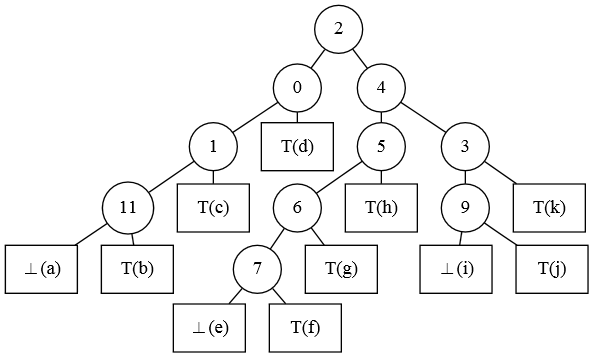
\includegraphics[width=.5\linewidth]{bsp-example-b.png}}%
	%
	\\\vspace{4mm}
	%
	\subfigure[]
	{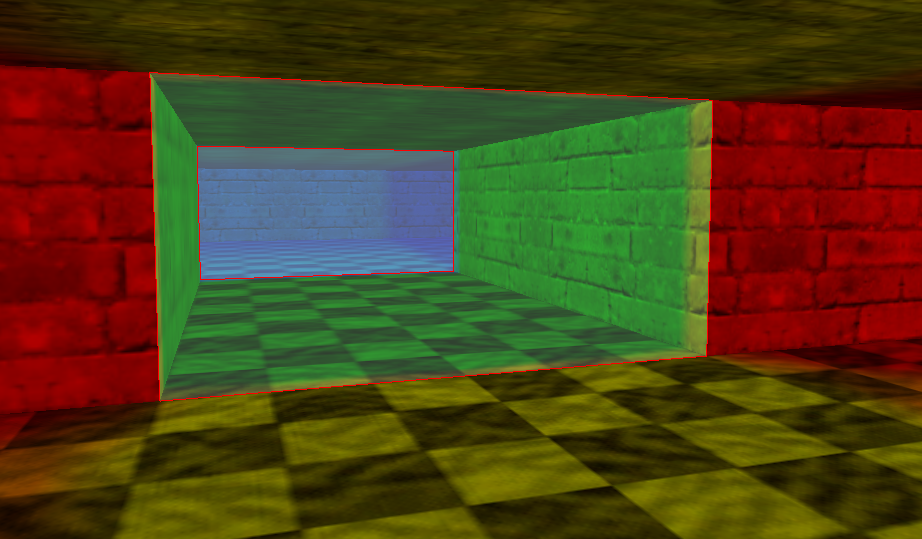
\includegraphics[width=.5\linewidth]{bsp-example-c.png}}%
\caption{A BSP example for a simple 2D world with two rooms, connected by a corridor: (a) shows a top-down view of the world, where the arrows represent the facings of the world polygons and the dashed lines represent the split planes chosen when constructing the BSP in (b); (b) shows the BSP tree that is constructed for the world based on the chosen split planes; (c) shows what a 3D version of the world looks like in \emph{hesperus}, with portals (doorways) rendered as translucent polygons to illustrate the boundaries between the empty leaves (a, e and i) of the BSP. (Note that the 3D version actually has additional floor and ceiling polygons, but we ignore that here for the purposes of explanation.)}
\label{fig:bsp-example}
\end{stusubfig}
%---

Binary space partitioning is a technique for representing n-dimensional space as a binary tree (known as a BSP tree) by recursively dividing it into two using \emph{hyperplanes} (the n-dimensional generalisation of planes). It was originally introduced by Fuchs et.\ al \cite{fuchs80} in 1980, and saw widespread use in first-person games of the \emph{Quake} era (e.g.~see \cite{abrash97}) as a way of representing 3D polygonal game worlds, most notably because it provided a way of rendering a world's polygons in either back-to-front or front-to-back order \cite{fuchs80,gordon91} without the need for a z-buffer on the graphics card (z-buffers once used to be quite costly). As graphics cards have matured, commercial games have moved away from binary space partitioning as a rendering approach, because traversing a BSP tree is relatively slow in comparison to simply throwing large numbers of triangles at the graphics card and letting the z-buffer handle the rendering order, but BSP trees remain interesting as a basis for collision detection and constructive solid geometry techniques \cite{ericson05,lysenko08}.

An example BSP tree is shown in Figure~\ref{fig:bsp-example}. Each node of the tree represents a convex subspace of the world being partitioned; moreover, the leaves of the tree represent a \emph{partition} of the entire space, i.e.~they are mutually disjoint and their union is equal to the space. Each branch node has an associated split plane (a line with facing in 2D) that divides the subspace represented by the node in two. Each leaf node contains the polygons (line segments in 2D) that fall within the subspace it represents, and carries a flag that indicates whether the subspace represented by the leaf is empty (i.e. navigable by an agent, denoted as $\bot$) or solid (non-navigable, denoted as $\top$). The BSP tree as a whole can be used to decide whether or not any given point in the world lies in empty or solid space in $O(h)$ time, where $h$ is the height of the tree, by the simple means of classifying the point against the split planes in the tree, starting from the root, and recursing down the relevant side of the tree at each stage until hitting a leaf.

Constructing a BSP tree for a polygonal world is also done recursively, starting from the set of all the polygons in the world. At each recursive step, one of the current set of polygons whose plane has not been used further up the tree is chosen as the \emph{split polygon}, and its plane is used to split the other polygons into two sets, one of polygons that are in front of the plane and one of those that are behind it. (If no suitable split polygon can be found, then we create a leaf of the tree to contain the current set of polygons and return.) If a polygon straddles the plane, it is split, with its two halves being placed in the appropriate sets. If a polygon lies on the plane, it is put into either the front or back set based on the orientation of its normal with respect to the plane. The two sets of polygons are then processed recursively to construct the subtrees of the current node. Finally, a branch node is constructed from the split plane and the two subtrees.

An extremely detailed description of BSP construction, together with diagrams that clarify precisely how the process works, can be found in \cite{golodetz06}; readers may additionally wish to take a look back at a previous article I wrote for \emph{Overload} that also discussed BSP construction \cite{golodetzoverload08aug}.

\section{Onion BSPs}
\label{sec:onionbsps}

%---
\begin{stusubfig}{!t}
	\subfigure[]
	{
	\begin{picture}(250,50)
		\thicklines
		\dashline{4}(0,35)(35,35)
		\dashline{4}(0,165)(35,165)
		\dashline{4}(215,165)(250,165)
		\dashline{4}(215,25)(215,0)
		\dashline{4}(35,75)(75,75)
		\dashline{4}(175,75)(215,75)
		\dashline{4}(35,125)(75,125)
		\dashline{4}(175,125)(215,125)
		\put(122.5,180){a}
		\put(230,97.5){b}
		\put(122.5,15){c}
		\put(15,97.5){d}
		\put(122.5,140){e}
		\put(190,97.5){f}
		\put(122.5,57.5){g}
		\put(57.5,97.5){h}
		\put(122.5,97.5){i}

		\color{red}
		\put(35.4,35.4){\framebox(179.2,129.2){}}
		\put(125,35){\vector(0,1){10}}		\put(130,37.5){2}
		\put(125,165){\vector(0,-1){10}}	\put(130,155){0}
		\put(35,100){\vector(1,0){10}}		\put(37.5,105){3}
		\put(215,100){\vector(-1,0){10}}	\put(207.5,105){1}
		\color{green}
		\put(75.4,75.4){\framebox(99.2,49.2){}}
		\put(125,75){\vector(0,1){10}}		\put(130,77.5){6}
		\put(125,125){\vector(0,-1){10}}	\put(130,115){4}
		\put(75,100){\vector(1,0){10}}		\put(77.5,105){7}
		\put(175,100){\vector(-1,0){10}}	\put(167.5,105){5}
		\color{black}
	\end{picture}
	}
	%
	\hspace{12mm}%
	%
	\subfigure[]
	{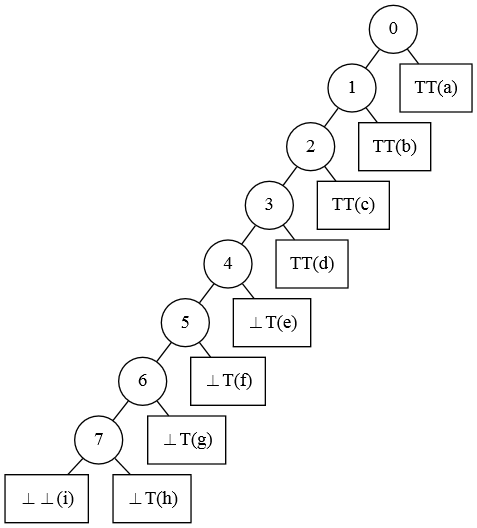
\includegraphics[width=.35\linewidth]{onion-example.png}}%
\caption{An example 2D world (a) and one possible onion BSP for it (b). The coloured lines (red and green) denote two separate configuration spaces. Their polygons (shown as numbered, oriented line segments) are compiled into the same onion BSP as shown. Individual leaves (labelled with letters) can be empty ($\bot$) in one space and solid ($\top$) in another, e.g.~leaf $e$ is empty in the red space but solid in the green one.}
\label{fig:onion-example}
\end{stusubfig}
%---

As mentioned in the previous section, standard BSP trees can be used to determine whether individual points are in empty or solid space; moreover, as will be seen later, this extends to line segments -- there is a relatively straightforward BSP algorithm that will allow us to find the first transition point at which a line segment crosses from empty to solid space. This can form the basis for a simple collision detection scheme for \emph{point-based} agents -- at each frame, we can test the line segment representing an agent's proposed movement for that frame against the tree, taking the first transition point as the point of collision if the agent tries to walk into a wall.

Unfortunately, however, most agents in 3D games are not point-based, so we need a way to handle objects with extent. The way I describe here is due to van Waveren \cite{vanwaveren01} and uses the notion of configuration spaces I described in \cite{golodetzoverload13oct}. An alternative, similar approach, that works by modifying a normal BSP at runtime, is discussed in \S\ref{sec:discussion}. Both of the approaches described are based on the same principle -- that performing collision detection between an object with extent and the world is equivalent to performing collision detection between a point at the centre of the object and a copy of the world that has been suitably expanded in accordance with the size of the object.

The van Waveren approach is an offline method designed for brush-based 3D environments (that is, environments built up by combining simple, convex polyhedra). Agents are represented by axis-aligned bounding boxes (AABBs); each class of agent may have multiple AABBs for different poses (e.g.~standing or crouching). At level compilation time, the brushes of the environment are expanded for each AABB and the faces of the expanded brushes are unioned together to form an expanded world for that AABB. Each of these expanded worlds can be compiled into a BSP tree, allowing us to perform collision detection for an object represented by the corresponding AABB. However, maintaining multiple BSP trees is inconvenient because then objects that are in the same physical location but have different sizes cannot be resolved to a leaf in any particular tree -- we would much prefer to have a single tree that represents all of the information available.

We can achieve this by constructing a different type of BSP tree that I call an \emph{onion BSP}\footnotemark{}. Onion BSPs are a generalisation of standard BSPs in which we replace the empty/solid flag in each leaf node with a vector of flags indicating whether the leaf is empty/solid in each configuration space associated with an AABB. Thus, a leaf might be solid in the configuration space corresponding to an agent's standing AABB, but empty in the space corresponding to its crouching AABB, indicating that the agent may traverse the area only whilst crouching. Figure~\ref{fig:onion-example} shows two configuration spaces generated for an example world (the original, unexpanded world is not shown) and an onion BSP that might be generated for it.

\footnotetext{For the interested reader, the name `onion BSP' comes from the idea that the expanded worlds look rather like the layers of an onion when superimposed in an image. This analogy is not strictly accurate, because the various different AABBs will not in general nest inside each other, but the name is nevertheless both suggestive and convenient.}

\subsection{The Compilation Process}

Onion BSP compilation is in principle much the same as BSP compilation (see \S\ref{sec:bsps}), but slightly trickier because we have to test the solidity of each leaf in each configuration space rather than getting it for free as part of the compilation process. An explanation of this testing process is deferred to the next section, but it also has an impact on the main part of the compilation. In particular, the test involves checking an arbitrary point in the leaf for solidity in each configuration space (the solidity of any point in the leaf is guaranteed to be the same as that of the entire leaf), so we will need (a) a way of determining an arbitrary point in a leaf, and (b) a way of testing a point for solidity in a configuration space. As will be seen, determining an arbitrary point in a leaf will involve knowing the set of split planes on the path from the root of the tree to the leaf, so these should be maintained during compilation.

The resulting main compilation process is shown in Listings~\ref{code:build-tree} and \ref{code:build-subtree}. The key thing to note is the way in which a set of split planes is maintained in order to facilitate solidity testing -- we add the current split plane to the set before each recursive call to \texttt{build\_subtree} and remove it again afterwards, so that whenever we reach a leaf it will contain precisely those split planes on the path from the root of the tree to the leaf. Note that orientation is important, so the current split plane must be reversed when recursing into the right-hand subtree.

%---
\begin{stulisting}[!t]
\caption{Building an Onion Tree}
\label{code:build-tree}
\lstinputlisting[style=Default]{build-tree.lst}
\end{stulisting}
%---

%---
\begin{stulisting}[!t]
\caption{Building an Onion Subtree}
\label{code:build-subtree}
\lstinputlisting[style=Default]{build-subtree.lst}
\end{stulisting}
%---

\subsection{Determining Leaf Solidity}

A \emph{solidity descriptor} for a leaf in an onion BSP is a list of bits indicating whether the leaf is empty or solid in each configuration space for which we compiled the BSP. It is common for a leaf to be empty in one configuration space and solid in another -- for example, a leaf might be empty in the configuration space corresponding to the crouch pose of an agent, but solid in the configuration space corresponding to the standing pose, indicating that the agent can traverse the leaf whilst crouching but not whilst standing (e.g.~think of a low tunnel). To determine a leaf's solidity descriptor, we find an arbitrary point in the leaf and check its solidity in each configuration space in turn; the resulting empty/solid results are combined to form the full solidity descriptor. To test points' solidity in a configuration space, we build a normal BSP tree (called a \emph{map tree} in the code) for the space at the start of the compilation process and later classify points with regard to it. The top-level process to determine leaf solidity is shown in Listing~\ref{code:determine-leaf-solidity}.

%---
\begin{stulisting}[!t]
\caption{Determining Leaf Solidity}
\label{code:determine-leaf-solidity}
\lstinputlisting[style=Default]{determine-leaf-solidity.lst}
\end{stulisting}
%---

\subsubsection{Finding an Arbitrary Leaf Point}

To find an arbitrary point in a leaf, recall that each leaf represents a convex subspace of the world. Our first intuition might be to create an explicit representation of the leaf as a convex polyhedron and then compute the average of the midpoints of the polyhedron's faces as our point. This does in fact work perfectly for fully-bounded leaves (see Figure~\ref{?}(a)), but unfortunately fails for unbounded ones (see Figure~\ref{?}(b)). Fortunately, in practice, there is an easy solution to this problem: we can simply stipulate that the world we are representing is bounded by an inward-facing box, thereby ensuring that every leaf is bounded (see Figure~\ref{?}). This is clearly a reasonable assumption in the context of representing a 3D world, since it would not be meaningful for such a world to be infinite. (The interested reader may wish to take a look at \cite{seidel91}, where a similar approach is taken to deal with unboundedness in a related linear programming problem.)

The algorithm itself is shown in Listing~\ref{code:arbitrary-leaf-point}. It is called with the set of ancestor planes leading down to the given leaf in the tree (recall that these are maintained as part of the top-level compilation process). These are augmented with the planes of the inward-facing box that we are assuming bounds the world. We then construct an extremely large polygon on each of the planes in turn, and clip it to the other planes (see \cite{hesperus} for the implementation details). The set of polygons that results forms a convex polyhedron representing the (bounded) leaf. As previously stated, we finally compute the midpoint of each face of the polyhedron and average them to produce an arbitrary point that is guaranteed to be inside the leaf.

%---
\begin{stulisting}[!t]
\caption{Finding an Arbitrary Leaf Point}
\label{code:arbitrary-leaf-point}
\lstinputlisting[style=Default]{arbitrary-leaf-point.lst}
\end{stulisting}
%---

\section{Collision Detection}
\label{sec:collisiondetection}

Having constructed an onion BSP for the world, it is now possible to perform collision detection against it for objects with a specific AABB, using a variant of the `find first transition' algorithm mentioned in \S\ref{sec:onionbsps}. The algorithm works as shown in Listing~\ref{?}. TODO

\section{Discussion}
\label{sec:discussion}

TODO: \cite{melax00}

\section{Conclusions}
\label{sec:conclusions}

TODO

\section{Acknowledgements}

TODO

%
% Detecting Object-Object Collisions using Minkowski Portal Refinement
% A Simple Physics Engine for 3D Games
% Agent Localisation and Movement in 3D Environments
%

\clearpage

%\nocite{*}

\bibliographystyle{plain}
\bibliography{onionbsp}

\end{document}
